\documentclass{article}

\usepackage[preprint]{neurips_2022}

\usepackage[utf8]{inputenc}
\usepackage{hyperref}
\usepackage{url}
\usepackage{booktabs}
\usepackage{amsmath}
\usepackage{amsfonts}
\usepackage{microtype}
\usepackage{xcolor}
\usepackage{graphicx}

\title{GraphRAG for Multi-Hop Question Answering with Dense, Graph Neural, and PCST Retrieval}

\author{%
  Nikhil Juluri \quad Chinmay Kawle \\
  Department of Computer Science \\
  University of Illinois at Chicago \\
  \texttt{njulu@uic.edu} \quad
  \texttt{ckawl@uic.edu} \\
}

\begin{document}

\maketitle

\begin{abstract}
Retrieval-augmented generation systems often treat retrieval as an independent nearest-neighbor search problem, even when answering requires assembling evidence from multiple related documents. This report describes a GraphRAG implementation for HotpotQA-style multi-hop question answering. The system loads each question with its local distractor context, chunks documents, embeds chunks with BGE, constructs question-local hybrid graphs, and compares dense retrieval, dense-guided PCST retrieval, GraphSAGE retrieval, dense--GraphSAGE fusion, and fusion-guided PCST retrieval. Evaluation uses 300 HotpotQA train examples and an LLM answer-generation protocol scored by exact match and token F1. Dense--GraphSAGE fusion obtains the best overall answer score among the evaluated modes, with 0.6833 exact match and 0.7580 F1, improving over dense retrieval on bridge questions while slightly reducing comparison-question performance. PCST variants are implemented and useful for studying graph-constrained evidence expansion, but the current LLM evaluation does not show an end-to-end gain over the fusion retriever.
\end{abstract}

\section{Introduction}

Multi-hop question answering requires retrieving evidence chains rather than isolated passages. In HotpotQA, a bridge question may require using one entity to find another supporting article, while a comparison question may require retrieving and contrasting two entities \citep{yang2018hotpotqa}. Standard dense retrieval can recover semantically similar chunks, but it does not explicitly model relationships among chunks from the same title, adjacent context, keyword overlap, or semantic neighborhoods.

This project studies a compact GraphRAG pipeline in which retrieval is performed over question-local context graphs. The implementation builds on retrieval-augmented generation (RAG) \citep{lewis2020rag}, dense passage retrieval ideas \citep{karpukhin2020dpr}, and graph neural networks \citep{hamilton2017graphsage}. It evaluates whether graph-aware ranking and graph-constrained expansion improve downstream LLM answer quality.

The main contributions of the report are:
\begin{itemize}
  \item a faithful description of the implemented HotpotQA preprocessing, chunking, dense retrieval, hybrid graph construction, Query-Aware GraphSAGE scoring, fusion retrieval, and PCST-style expansion modules;
  \item an end-to-end answer evaluation of five retrieval modes using identical 300-question LLM evaluation files; and
  \item an analysis separating bridge and comparison questions, where the fusion model improves bridge answer F1 over dense retrieval but does not dominate every category.
\end{itemize}

\section{Related work}

Retrieval-augmented generation combines an external retriever with a conditional generator so that generated answers are grounded in retrieved evidence \citep{lewis2020rag}. Sparse lexical retrieval, including BM25 \citep{robertson2009probabilistic}, remains a strong baseline in many open-domain QA settings because exact term matching can recover rare entities. The current evaluated code path does not implement a BM25 baseline; the repository focuses on dense and graph-based variants, while retaining ``FAISS-only'' labels for dense nearest-neighbor retrieval.

Dense Passage Retrieval (DPR) showed that learned dense encoders can outperform traditional sparse retrieval for open-domain QA when trained with question--passage supervision \citep{karpukhin2020dpr}. This project uses SentenceTransformers with the BGE encoder rather than a DPR-trained dual encoder, but follows the same scoring pattern: encode the query and candidate chunks, normalize vectors, and rank by inner product.

Graph retrieval methods add structure to candidate evidence. GraphSAGE aggregates local neighborhood information and supports inductive node classification \citep{hamilton2017graphsage}; in this project, a Query-Aware GraphSAGE model predicts supporting chunk probabilities on per-question graphs. Prize-Collecting Steiner Tree (PCST) methods select valuable nodes while penalizing traversal cost \citep{goemans1995pcst}. The implementation uses a greedy multi-seed PCST-style expansion rather than an exact PCST solver, so we describe it as PCST-inspired graph selection.

\section{Methodology}

\subsection{Dataset and preprocessing}

The loader in \texttt{graphrag\_env/src/loading.py} uses the Hugging Face \texttt{hotpot\_qa} dataset with the \texttt{distractor} configuration. Each returned example stores the question id, question, answer, type, difficulty level, supporting fact titles and sentence ids, and the local context documents. Context documents are represented as LangChain \texttt{Document} objects with metadata including title, question id, question type, context index, source, and a Boolean \texttt{is\_supporting} field.

\subsection{Chunking and embedding}

The chunking module uses a \texttt{RecursiveCharacterTextSplitter} with chunk size 300, overlap 50, and separators ordered from paragraphs down to characters. Very short documents below the minimum text length are skipped. Each chunk receives a stable id of the form \texttt{question\_id::title::chunk\_index}, plus chunk index and text-length metadata.

The embedding module encodes chunks with \texttt{BAAI/bge-base-en-v1.5}. Embeddings are generated per question, converted to NumPy arrays, and normalized. Query encoding uses the BGE search prefix:
\begin{quote}
\small \texttt{Represent this sentence for searching relevant passages:}
\end{quote}
Dense scores are cosine similarities implemented as inner products between normalized query and chunk vectors.

\subsection{Dense retrieval}

Dense retrieval ranks chunks independently:
\begin{equation}
s_{\mathrm{dense}}(q,c_i) = \mathbf{e}(q)^\top \mathbf{e}(c_i),
\end{equation}
where both embeddings are normalized. The top-$k$ chunks are returned and their titles are deduplicated in rank order for support-title recall evaluation. In the application and evaluation labels this mode is called ``FAISS-only retrieval'', although the inspected core evaluation function computes exact dense inner products over the local candidate set; optional FAISS acceleration appears in the application service code.

\subsection{Sparse/BM25 retrieval}

BM25 is relevant as a lexical baseline for multi-hop QA, but no BM25 or \texttt{rank\_bm25} implementation is present in the inspected retrieval and evaluation modules. Therefore, this report does not include BM25 numbers. A future sparse or hybrid sparse--dense baseline could score chunks with BM25 and combine lexical and dense evidence as
\begin{equation}
s(q,c_i)=\alpha s_{\mathrm{dense}}(q,c_i)+(1-\alpha)s_{\mathrm{BM25}}(q,c_i),
\end{equation}
after appropriate normalization. This equation is included as a planned extension, not as an evaluated component.

\subsection{Graph construction}

The hybrid graph builder constructs one undirected NetworkX graph per question. Nodes correspond to chunks. Edges are added for four implemented relations: chunks from the same title, adjacent chunks within a title, semantic $k$-nearest-neighbor links using chunk embedding similarity, and keyword-overlap links after stopword filtering. The default graph settings in the evaluation scripts use semantic $k=2$, semantic minimum similarity 0.40, and keyword-overlap threshold 3.

The cached 10,000-example artifact contains 263,113 global chunks. Across these question-local graphs, the average graph has 26.31 nodes and 106.69 edges, with 4.13 supporting chunk nodes on average. Edge construction is dominated by keyword-overlap and semantic-neighborhood relations: the artifact contains 794,131 keyword-overlap edge labels, 376,596 semantic-kNN labels, 348,207 same-title labels, and 165,605 adjacent-chunk labels. These statistics are useful because they show that the GNN and PCST modules operate over small local graphs rather than one monolithic corpus graph.

\begin{figure}[t]
  \centering
  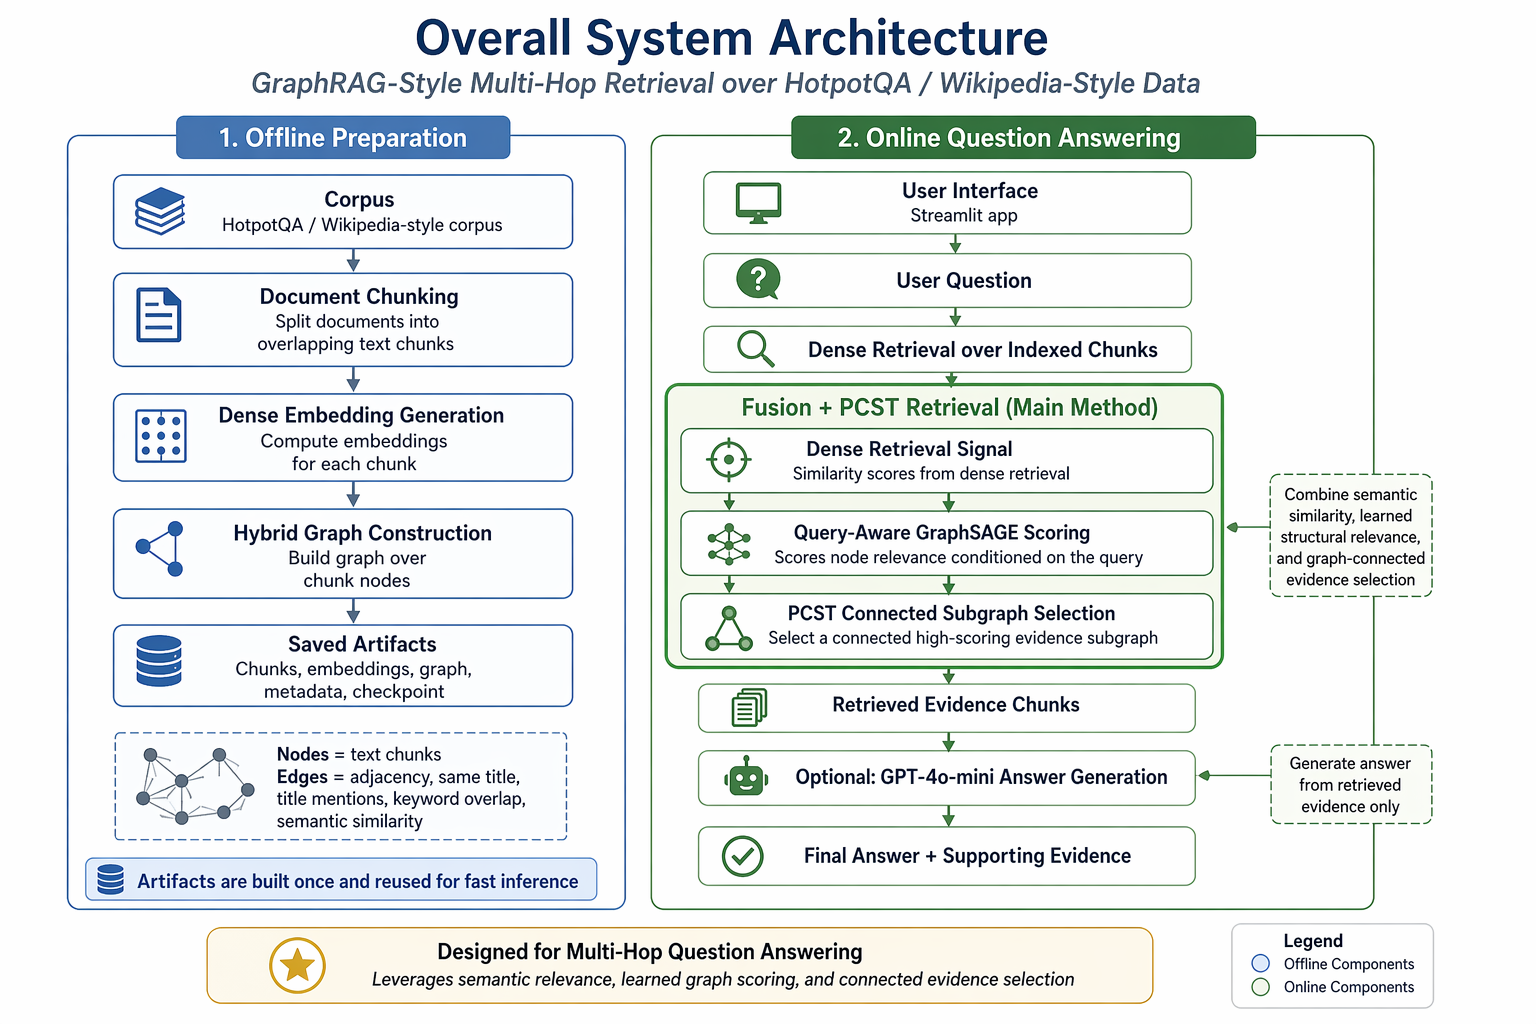
\includegraphics[width=0.92\linewidth]{figures/overall-system-architecture-fusion-pcst.png}
  \caption{Implemented GraphRAG architecture. The system loads HotpotQA examples, chunks and embeds local context, builds hybrid graphs, and evaluates dense, GNN, fusion, and PCST-style retrieval before answer generation.}
  \label{fig:architecture}
\end{figure}

\subsection{GNN-based retrieval}

The GNN module implements a Query-Aware GraphSAGE model with two \texttt{SAGEConv} layers, batch normalization, ReLU activations, dropout, a residual connection after the first layer, and a linear binary classifier. For each chunk node, the input feature vector concatenates the chunk embedding, repeated query embedding, and dense cosine similarity:
\begin{equation}
\mathbf{x}_i = [\mathbf{e}(c_i); \mathbf{e}(q); s_{\mathrm{dense}}(q,c_i)].
\end{equation}
Labels are derived from the chunk metadata: supporting chunks are positive, all other local chunks are negative. Training uses binary cross-entropy with a global positive-class weight computed from the training split, Adam, gradient clipping, and early stopping on validation loss. GNN retrieval ranks chunks by sigmoid node probability.

\subsection{Fusion and PCST retrieval}

Fusion retrieval combines normalized dense scores and normalized GNN probabilities:
\begin{equation}
s_{\mathrm{fusion}}(q,c_i)=\lambda s_{\mathrm{dense}}^{\mathrm{norm}}(q,c_i)
 +(1-\lambda)s_{\mathrm{gnn}}^{\mathrm{norm}}(q,c_i).
\end{equation}
The LLM evaluation uses $\lambda=0.5$ for fusion and PCST modes.

Two PCST-style variants are implemented. Dense-guided PCST seeds the greedy expansion with dense scores. The main PCST mode first computes dense--GNN fusion scores, selects multiple high-prize seed nodes, expands through graph neighbors according to a prize-minus-edge-cost heuristic, preserves the top fusion anchors, adds a small PCST bonus to selected nodes, and applies a title-diversity bonus during final ranking. This is a practical, greedy approximation of the PCST objective rather than an exact solver.

\section{Experimental setup}

\subsection{Data and retrieval settings}

The LLM evaluation files cover 300 HotpotQA train examples, with 237 bridge questions and 63 comparison questions. Retrieval depth is top 5. The graph-aware scripts mirror the train/validation split from GNN training for retrieval recall experiments, while the LLM result JSON files used here report end-to-end answer quality for 300 examples per mode.

\subsection{Answer generation and metrics}

The evaluation script retrieves chunks, builds a context prompt from the top retrieved chunks, and asks \texttt{gpt-4o-mini} at temperature 0 to return a short JSON answer using only the provided context. If no API key is configured, the script contains a heuristic fallback answerer, but the result JSON files used in this report are the saved evaluation artifacts. Predictions are scored with HotpotQA-style normalized exact match (EM) and token F1. Metrics are reported overall and separately for bridge and comparison questions.

\subsection{Inference timing protocol}

We additionally measure retrieval-only inference time using cached artifacts. Timing excludes offline data loading, chunking, embedding generation for passages, graph construction, GNN training, model loading, and LLM answer generation. Each measurement includes the online query embedding and the retrieval computation required by that mode. We time 500 randomly sampled cached HotpotQA graph examples after warmup queries on the local arm64 development machine.

\section{Results}

Table~\ref{tab:retrieval-results} reports retrieval-side support-title recall from the repository's result-table generation script. Unlike the LLM answer table, the dense row uses all 10,000 examples, while the graph-aware rows use the shared 2,000-question held-out split created by the GNN pipeline. The main PCST variant has the highest support recall@5 in this retrieval-only evaluation, reaching 0.8045 overall and 0.8014 on bridge questions. This shows that PCST expansion can improve evidence-title coverage even when its downstream LLM answer score is weaker.

\begin{table}[t]
  \centering
  \small
  \caption{Retrieval evaluation with support recall@5 (SR@5) and partial support recall@5 (P-SR@5). Dense is reported on 10,000 examples; graph-aware modes are reported on the 2,000-question held-out split.}
  \label{tab:retrieval-results}
  \resizebox{\linewidth}{!}{%
  \begin{tabular}{lrrrrrrr}
    \toprule
    Retriever & $n$ & Overall SR@5 & Overall P-SR@5 & Bridge SR@5 & Bridge P-SR@5 & Comp. SR@5 & Comp. P-SR@5 \\
    \midrule
    Dense (FAISS-only label) & 10000 & 0.7752 & 0.9898 & 0.7618 & 0.9898 & \textbf{0.8330} & \textbf{0.9899} \\
    Dense-guided PCST & 2000 & 0.7430 & 0.9855 & 0.7288 & 0.9852 & 0.8048 & 0.9866 \\
    GNN retrieval & 2000 & 0.7675 & 0.9870 & 0.7589 & 0.9871 & 0.8048 & 0.9866 \\
    Dense + GraphSAGE fusion & 2000 & 0.7940 & 0.9915 & 0.7897 & 0.9926 & 0.8128 & 0.9866 \\
    Dense + GraphSAGE + PCST & 2000 & \textbf{0.8045} & \textbf{0.9925} & \textbf{0.8014} & \textbf{0.9939} & 0.8182 & 0.9866 \\
    \bottomrule
  \end{tabular}
  }
\end{table}

Table~\ref{tab:llm-results} reports answer-level metrics from the root-level JSON result files. Dense--GraphSAGE fusion is the best overall mode among the evaluated files, with 0.6833 EM and 0.7580 F1. The gain is concentrated on bridge questions: bridge F1 improves from 0.7216 for dense retrieval to 0.7564 for fusion. Comparison questions show the opposite pattern, where dense and GNN retrieval have higher EM than fusion, and dense retrieval has the highest comparison F1.

\begin{table}[t]
  \centering
  \small
  \caption{LLM answer evaluation on 300 HotpotQA examples. EM and F1 are computed after answer normalization.}
  \label{tab:llm-results}
  \resizebox{\linewidth}{!}{%
  \begin{tabular}{lrrrrrr}
    \toprule
    Retriever & Overall EM & Overall F1 & Bridge EM & Bridge F1 & Comp. EM & Comp. F1 \\
    \midrule
    Dense (FAISS-only label) & 0.6600 & 0.7338 & 0.6414 & 0.7216 & \textbf{0.7302} & \textbf{0.7797} \\
    Dense-guided PCST & 0.6500 & 0.7193 & 0.6371 & 0.7117 & 0.6984 & 0.7480 \\
    GNN retrieval & 0.6600 & 0.7380 & 0.6414 & 0.7297 & \textbf{0.7302} & 0.7692 \\
    Dense + GraphSAGE fusion & \textbf{0.6833} & \textbf{0.7580} & \textbf{0.6751} & \textbf{0.7564} & 0.7143 & 0.7639 \\
    Dense + GraphSAGE + PCST & 0.6500 & 0.7177 & 0.6329 & 0.7027 & 0.7143 & 0.7745 \\
    \bottomrule
  \end{tabular}
  }
\end{table}

\begin{table}[t]
  \centering
  \small
  \caption{Retrieval-only inference time per query in milliseconds over 500 measured examples. Timing excludes model/artifact loading and LLM answer generation.}
  \label{tab:latency}
  \begin{tabular}{lrrrr}
    \toprule
    Retriever & $n$ & Mean ms & P50 ms & P95 ms \\
    \midrule
    Dense & 500 & 19.85 & 17.01 & 38.44 \\
    Dense-guided PCST & 500 & \textbf{16.81} & 16.15 & 25.45 \\
    GNN retrieval & 500 & 16.97 & 16.15 & \textbf{25.31} \\
    Dense + GraphSAGE fusion & 500 & 33.84 & 31.84 & 52.59 \\
    Dense + GraphSAGE + PCST & 500 & 32.96 & 30.96 & 51.10 \\
    \bottomrule
  \end{tabular}
\end{table}

\begin{figure}[t]
  \centering
  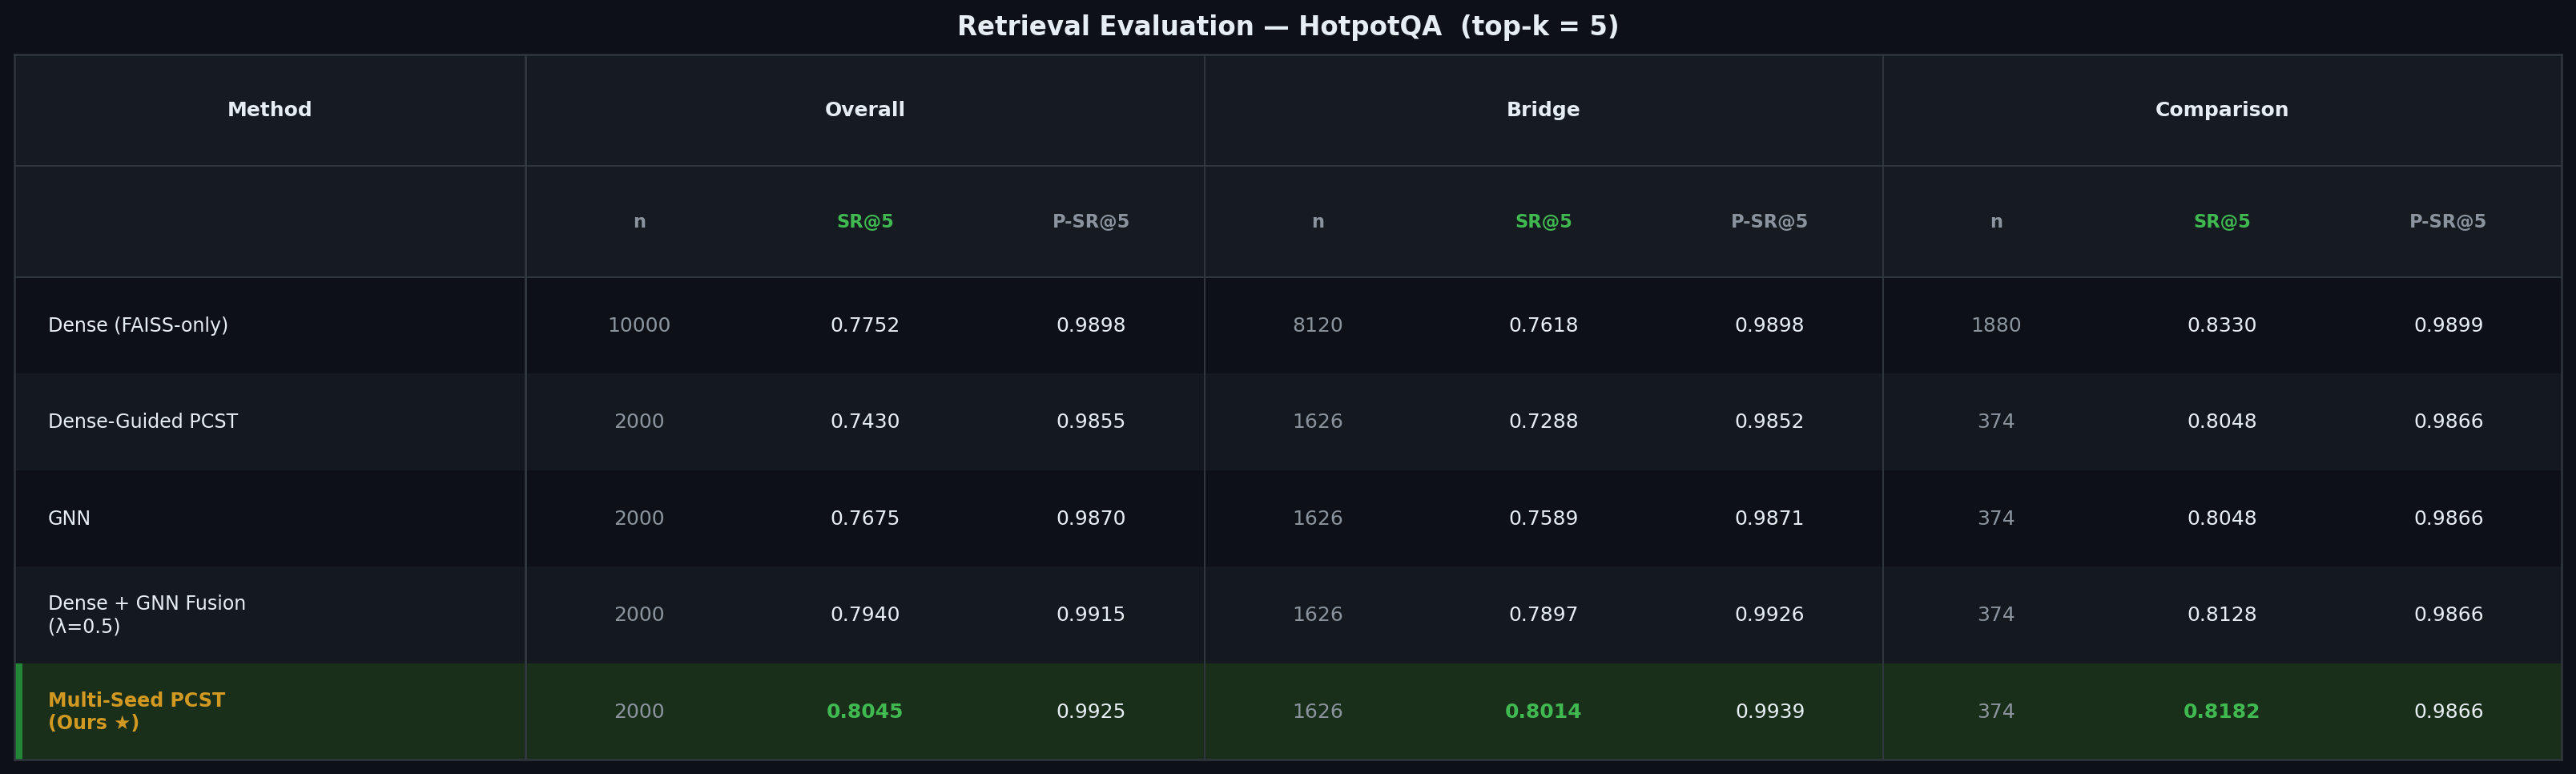
\includegraphics[width=\linewidth]{figures/retrieval_results_wide.png}
  \caption{Saved result visualization comparing answer EM and F1 across retrieval modes.}
  \label{fig:wide-results}
\end{figure}

\begin{figure}[t]
  \centering
  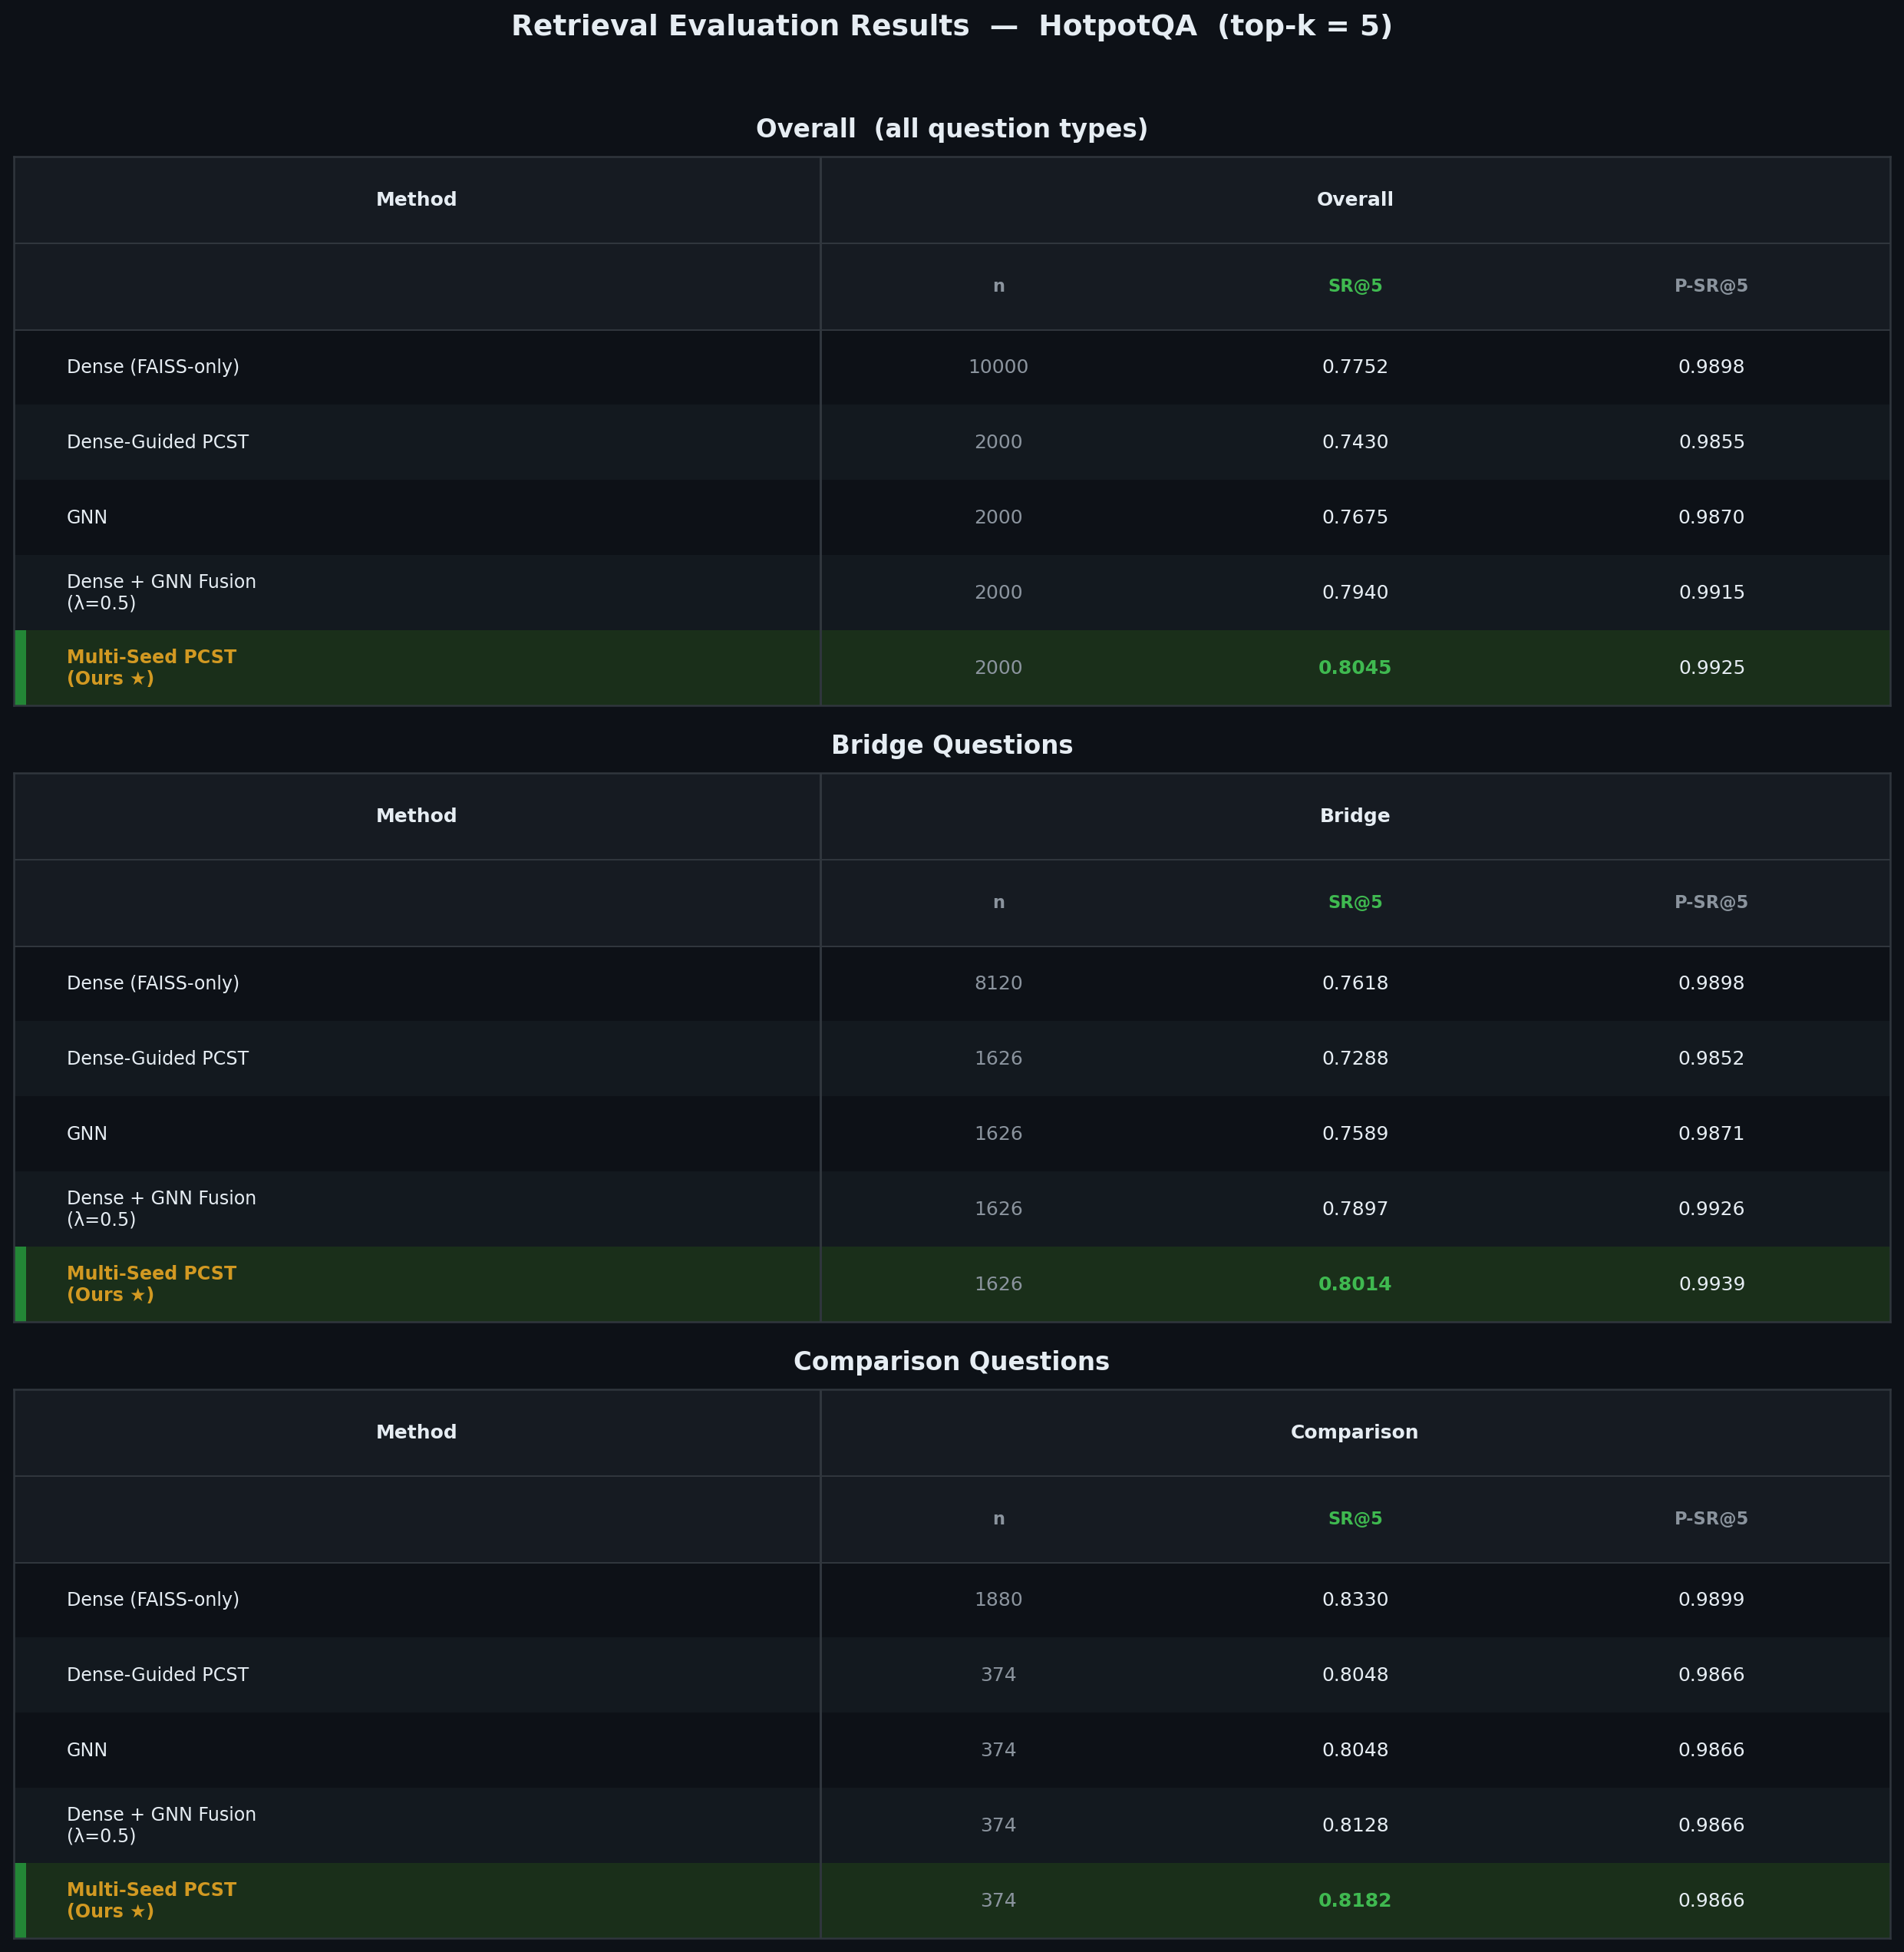
\includegraphics[width=0.95\linewidth]{figures/retrieval_results_tables.png}
  \caption{Tabular visualization of the LLM evaluation results included with the project assets.}
  \label{fig:result-tables}
\end{figure}

\subsection{Bridge versus comparison behavior}

Bridge questions benefit most from the learned fusion retriever. This matches the intended use of graph information: a GNN can use local structure and query-conditioned node features to promote chunks that are not merely individually similar to the query, while dense scores preserve strong semantic matches. The bridge improvement is modest but consistent across EM and F1 in the saved evaluation files.

Comparison questions are less clearly helped by graph expansion. Dense retrieval already tends to recover the two compared entities when the query names them explicitly, and graph-based reranking can introduce alternative titles that are structurally connected but less useful for direct comparison. The PCST main method has comparison F1 of 0.7745, close to dense retrieval, but its bridge degradation reduces overall performance.

\begin{table}[t]
  \centering
  \small
  \caption{Qualitative cases from the saved LLM evaluation JSONs. These examples illustrate why fusion improves bridge answers but graph expansion can still hurt downstream generation.}
  \label{tab:qualitative}
  \resizebox{\linewidth}{!}{%
  \begin{tabular}{p{0.17\linewidth}p{0.40\linewidth}p{0.13\linewidth}p{0.13\linewidth}p{0.13\linewidth}}
    \toprule
    Case & Question summary & Gold & Baseline output & Alternative output \\
    \midrule
    Fusion fixes dense & Nationality of James Henry Miller's wife & American & Dense: insufficient evidence & Fusion: American \\
    Fusion fixes dense & Origin of the music played by Die Rhoner Sauwantzt & United States & Dense: Hessen, Germany & Fusion: United States \\
    PCST hurts dense & Year of birth for the 2016 Marrakesh ePrix winner & 1988 & Dense: 1988 & PCST: 1984 \\
    Comparison noise & Whether Robert Fleischman and Jimmy Barnes share nationality & no & Dense: No & Fusion: insufficient evidence \\
    \bottomrule
  \end{tabular}
  }
\end{table}

\section{Discussion}

The strongest result is that simple score fusion is more reliable than replacing dense retrieval with a graph-only or graph-expanded ranking. Dense retrieval provides a robust semantic prior, while Query-Aware GraphSAGE contributes a learned estimate of support relevance. The implemented fusion equation is therefore an effective conservative combination.

The PCST-style methods are more mixed. Retrieval recall improves for the main PCST method, but answer quality drops relative to dense--GNN fusion. The code includes several safeguards: fallback filling when graph expansion stalls, preservation of top fusion anchors, a PCST bonus, and a title-diversity bonus. These choices make the method robust enough to return full result sets, but the qualitative examples suggest that graph expansion can still alter prompt composition in ways that move answer-critical context away from the generator or introduce confusable alternatives. This is especially costly when the generator receives only five chunks.

The figures and result table should also be interpreted as project-scale evidence rather than a benchmark claim. The evaluation uses 300 examples, one prompt template, one LLM, and one set of retrieval hyperparameters. The results are useful for guiding development, but not for claiming state-of-the-art performance.

\section{Limitations}

The current report has several implementation and evaluation limitations. First, BM25 is discussed as related work and a future baseline, but it is not implemented in the inspected retrieval code. Second, the PCST implementation is greedy and PCST-inspired rather than an exact prize-collecting Steiner tree solver. Third, the LLM evaluation depends on one model and one prompt format, and the saved JSON metrics do not include confidence intervals. Fourth, the answer evaluation is run on a 300-example subset of the HotpotQA train split rather than the official development set. Finally, graph construction is question-local over HotpotQA distractor contexts; global corpus retrieval behavior may differ from these controlled local-context experiments.

\section{Conclusion}

This GraphRAG project implements a practical multi-hop QA retrieval stack with dense retrieval, hybrid graph construction, Query-Aware GraphSAGE scoring, dense--GNN fusion, and PCST-style graph expansion. On the saved 300-question LLM evaluation, dense--GraphSAGE fusion provides the best overall answer quality and the clearest bridge-question improvement. The graph and PCST modules remain valuable for evidence-chain experiments, but the current results indicate that graph expansion needs careful calibration when only a small number of chunks reach the generator.

\section*{Reproducibility notes}

The paper can be compiled from the repository root with:
\begin{verbatim}
cd paper
pdflatex main.tex
bibtex main
pdflatex main.tex
pdflatex main.tex
\end{verbatim}
The metrics in Table~\ref{tab:llm-results} are taken from \texttt{llm\_eval\_results\_dense.json}, \texttt{llm\_eval\_results\_fusion.json}, \texttt{llm\_eval\_results\_gnn.json}, \texttt{llm\_eval\_results\_pcst.json}, and \texttt{llm\_eval\_results\_pcst\_dense.json} at the repository root.

\bibliographystyle{plainnat}
\bibliography{references}

\appendix
\section{NeurIPS checklist}

\begin{enumerate}
  \item For all authors: Do the main claims made in the abstract and introduction accurately reflect the paper's contributions and scope? \answerYes{} The report limits claims to the implemented pipeline and saved evaluation files.
  \item Did you describe the limitations of your work? \answerYes{} See the Limitations section.
  \item Did you discuss any potential negative societal impacts of your work? \answerNA{} This is a project report on retrieval methodology over an existing QA dataset.
  \item Did you include complete proofs for theoretical results? \answerNA{} The report contains no theoretical claims requiring proofs.
  \item Did you include the code, data, and instructions needed to reproduce the main experimental results? \answerYes{} The repository contains the code and saved result files; compile instructions are included above.
  \item Did you specify all training details relevant to the reported results? \answerYes{} The report summarizes chunking, embedding, graph construction, GraphSAGE features, optimization choices visible in the code, and LLM evaluation settings.
  \item Did you report error bars? \answerNo{} The saved JSON artifacts contain point estimates only.
  \item Did you include the compute resources used? \answerNo{} The inspected result files do not record hardware details.
  \item Did you describe dataset splits and preprocessing? \answerYes{} See Dataset and preprocessing and Experimental setup.
\end{enumerate}

\end{document}
